\chapter{Hash Table Implementation} % Write in your own chapter title
\label{Chapter3}
\lhead{Chapter 3. \emph{Hash Table Implementation}}

\section{Methodology}
Quadratic Probing for Hash tables is used to carryout basic operations on the data array. These basic operations and their working are as follows:

\subsection{Insertion}
First of all, a hash table of size 1.5 times the size of data is created and then the data from the array is inserted into hash table by computing hash function which is id \% table size. On collision the second hash function is calculated and the data is inserted at the appropriate position.

Time Complexity: \textbf{O(1) approaches to O(N)} \\
Space Complexity: \textbf{O(N)}

\subsection{Finding}
In order to find the data, hash function is calculated using the given id. If the required key is found the index of the cell is returned, else by using the formula of quadratic probing the next is cell checked and so on until an empty cell or the required key is reached.

Time Complexity: \textbf{O(N)} \\
Space Complexity: \textbf{O(N)}

\subsection{Sorted Traversal}
For sorted traversal 101, all the IDs of hash table are copied in an array, the array is sorted using quick sort algorithm. The sorted array is traversed, and for the given ID, its location is found in hash table and the data is printed

Sorting Algorithm Used: \textbf{Quick Sort O(log N)} \\
Time Complexity: \textbf{O(N log N)}\\ 
Space Complexity: \textbf{O(N)} \\

For simple sorted traversal, hash table is traversed, the minimum element is found and marked as found, and printed then the other minimum is found and printed and so on.
 Time Complexity: \textbf{O($N^2$)}\\ 
 Space Complexity: \textbf{O(N)} \\ 
\textit{Note: Sorted traversal time complexity is dependent upon sorting algorithm used.}\\
\subsection{Deletion}
Deletion is carried out by finding the cell in which the id to be deleted is present, then the cell is marked as deleted. 

Time Complexity: \textbf{O(1)} \\
Space Complexity: \textbf{O(N)}


\section{Execution Times and Memory Consumptions}
\begin{figure}[H]
	\centering
	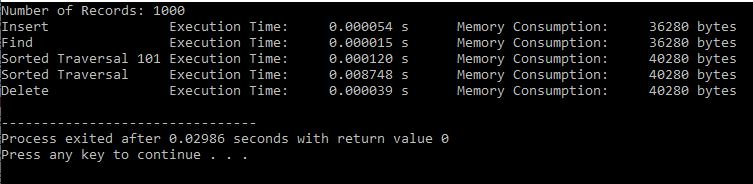
\includegraphics[scale =0.7]{./Figures/hash1000.jpg}
	\rule{35em}{0.5pt}
	\caption{Results for hash implementation with data size 1000.}
	\label{fig:Hash 1000}
\end{figure}

\begin{figure}[H]
	\centering
	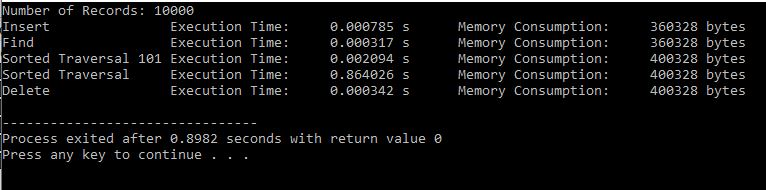
\includegraphics[scale =0.7]{./Figures/hash10000.jpg}
	\rule{35em}{0.5pt}
	\caption{Results for hash implementation with data size 10000.}
	\label{fig:Hash 10000}
\end{figure}

\begin{figure}[H]
	\centering
	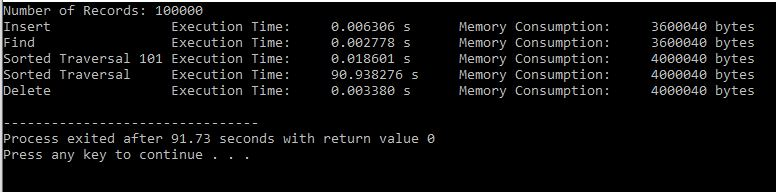
\includegraphics[scale =0.7]{./Figures/hash100000.jpg}
	\rule{35em}{0.5pt}
	\caption{Results for hash implementation with data size 100000.}
	\label{fig:Hash 100000}
\end{figure}

\begin{figure}[H]
	\centering
	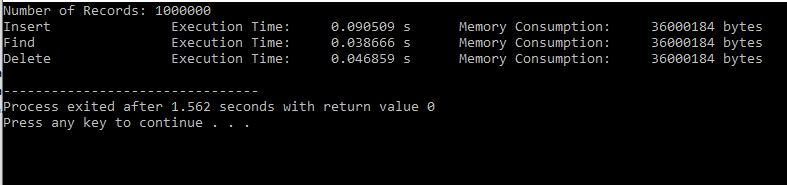
\includegraphics[scale =0.7]{./Figures/hash1000000.jpg}
	\rule{35em}{0.5pt}
	\caption{Results for hash implementation with data size 1000000.}
	\label{fig:Hash 1000000}
\end{figure}
